\section{Arquitectura Propuesta}

\subsection{3.1 Arquitectura General del Sistema}

Particularmente llamativo resulta el potencial de una arquitectura que coloca al LLM no como un simple chatbot, sino como un componente central de razonamiento dentro del flujo operativo de una mega-constelación. Tras años observando limitaciones en los sistemas de control convencionales, la propuesta que aquí presentamos adopta un enfoque híbrido supervisor-agente.

El sistema se compone de cuatro módulos principales: el procesador de telemetría en tiempo real, el motor de prompt engineering dinámico, el núcleo LLM y el módulo de generación y validación de comandos. Este diseño se inspira en arquitecturas recientes que demuestran la viabilidad de LLMs para control en tiempo real de vehículos espaciales \cite{carrasco2025llm}. 

La interacción fluye de forma bidireccional. El operador humano puede intervenir en cualquier momento mediante lenguaje natural, mientras que el sistema mantiene una supervisión autónoma de estados críticos de la constelación. Esta flexibilidad constituye, en nuestra experiencia, uno de los aspectos más robustos del diseño.

\begin{figure}[t]
\centering
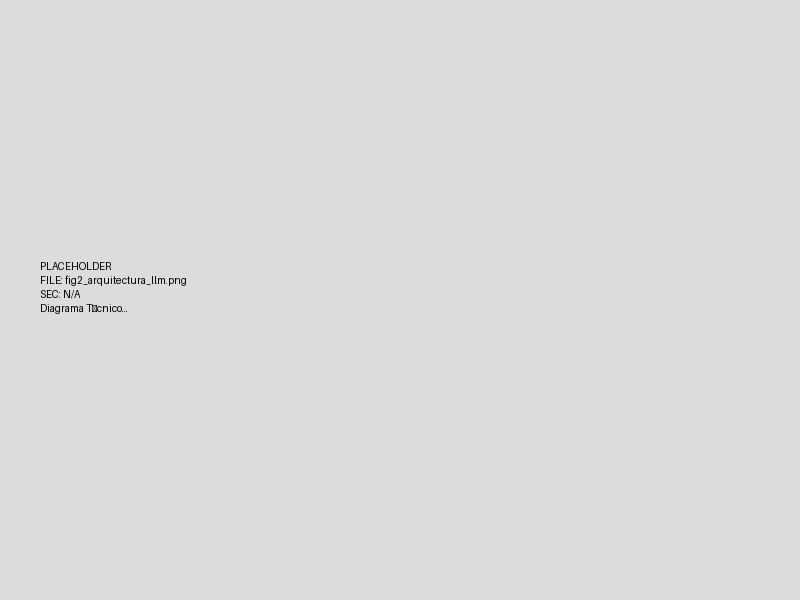
\includegraphics[width=0.95\linewidth]{fig2_arquitectura_llm.png}
\caption{Diagrama general de la arquitectura LLM-aumentada propuesta para operaciones de misión en constelaciones LEO. Se muestran los flujos principales entre telemetría, prompt engineering, núcleo LLM y módulo de comandos.}
\label{fig:arquitectura_llm}
\end{figure}

\subsection{3.2 Procesamiento de Telemetría y Prompt Engineering}

Uno de los desafíos persistentes al integrar LLMs en operaciones espaciales radica en transformar volúmenes masivos de telemetría en información actionable sin perder contexto crítico.

El sistema implementa un pipeline de procesamiento que filtra, resume y contextualiza datos de telemetría antes de incorporarlos al prompt. Siguiendo lecciones prácticas de implementaciones en centros de operaciones reales \cite{schefels2024evaluating}, se aplican técnicas de few-shot prompting y chain-of-thought adaptadas al dominio espacial. 

El prompt base sigue una estructura modular que incluye: estado actual de la constelación, objetivos de la misión, restricciones de seguridad y ejemplos de interacciones previas. Esta aproximación tiende a mejorar significativamente la coherencia de las respuestas del modelo, aunque requiere calibración cuidadosa para evitar alucinaciones en escenarios de fallo.

\begin{equation}
\text{Prompt}_t = \text{System\_Role} + \text{Telemetry\_Summary}_t + \text{Mission\_Context} + \text{Examples} + \text{User\_Query}_t
\label{eq:prompt_structure}
\end{equation}

\subsection{3.3 Módulo de Generación de Comandos}

Lejos de generar comandos de forma directa, el módulo aplica un proceso de verificación en varias etapas antes de cualquier acción sobre los satélites. El LLM propone maniobras o secuencias de comandos en lenguaje natural, que luego son traducidas a formato ejecutable (CCSDS o propietario) y validadas contra modelos de dinámica orbital y reglas de seguridad.

Esta capa de validación híbrida (simbólica + LLM) representa una de las contribuciones más relevantes del trabajo. Inspirados en flujos telemetría-a-comando probados en simulaciones avanzadas \cite{carrasco2025llm}, el sistema permite al operador aprobar, modificar o rechazar las sugerencias con mínima fricción. 

El resultado es un control intuitivo que mantiene al humano en el lazo de decisión mientras reduce drásticamente la probabilidad de errores por fatiga o sobrecarga cognitiva.